A CNN consists of some convolutional and subsampling layers optionally followed by fully connected layers. In this part, we introduce the layers used in our work.
\subsection{Convolutional Layer}
Convolutional Layer is the core building block of a Convolutional Network, and its output volume can be interpreted as holding neurons arranged in a 3D volume.
Natural images have the property of being "stationary" meaning that the statistics of one part of the image are the same as any other part. This suggests that the features that we learn at one part of the image can also be applied to other parts of the image, and we can use the same features at all locations. For example, some low-level features such as some special points or edges exist in many objects and can be used as the features for different types of objects.

Formally, given some original $h\times w$ input images $I$, we can train a small autoencoder from $a \times b$ kernel matrix. Also, we have to set other hyperparameters, stride $s$ and padding $p$. Stride defines the number of pixels the kernel should be moved in each step around the image $I$ and padding defines the number of rows/columns padded to the height and width of the original input (see Figure \ref{fig:cnn:conv}). 
Given a $a \times b$ kernel matrix $W^{(1)}$, bias $b^{(1)}$, padding $p$ and stride $s$, we can encode the original image $I$ as $f_{conv}=sigmod(W^{(1)}I_p+b^{(1)})$ for $I_p \in I$, giving us $f_{conv}$ (called feature map of $W^{(1)}$), a  $\left\lceil\frac{(h-a+2p)}{s}+1\right\rceil\times\left\lceil\frac{(w-b+2p)}{s}+1\right\rceil$ array of feature map. In general, for any specific input $I$ ($h \times w \times c$ array matrix) of a convolutional layer $L$, assuming we have $k$ such $a \times b \times c$ kernel matrix, its feature maps $f$ should be a $\left\lceil\frac{(h-a+2p)}{s}+1\right\rceil\times\left\lceil\frac{(w-b+2p)}{s}+1\right\rceil \times k$ array matrix with $f_{conv}^{(i)}=sigmod(W^{(i)}I_p+b^{(i)})$ for $I_p \in I$ and $i \in 1,\dots k$.

In real applications, small kernels ($3\times3$, $5\times5$ and $7\times7$) are preferred by many different CNN architectures \cite{krizhevsky2012imagenet} \cite{lecun1998gradient} \cite{simonyan2014very} \cite{zeiler2014visualizing}. Recent development of tiny $1\times1$ kernel shows an improvement on both accuracy and computational efficiency \cite{szegedy2014going}.
\begin{figure}
	\centering
	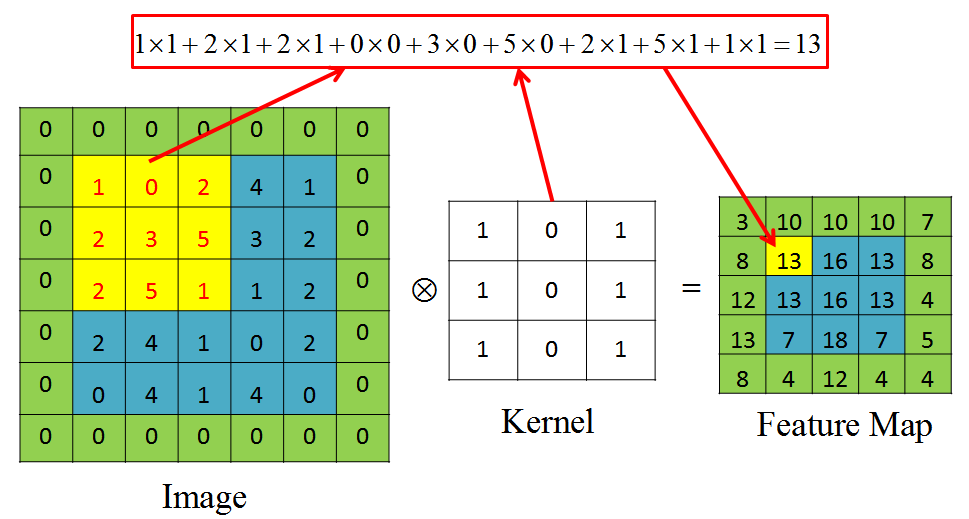
\includegraphics[scale=.6]{cnn/fig/conv.png}
	\caption{Convolution operation with $3\times3$ kernel, stride 1 and padding 1. $\otimes$ denotes the convolutional operator.} \label{fig:cnn:conv}
\end{figure}

\subsection{Pooling Layer}
Pooling layer is widely used in all kinds of CNN architecture for dimensional reduction and computational efficiency. 
After obtaining features maps using convolutional layer, we need to use them for classification. However, applying the feature maps from the convolutional layer for classification would be a computational challenge. Consider for instance images of size $96\times96$ pixels, and suppose we have learned 400 features over $8\times8$ inputs. Each convolution results in an output of size $(96-8+1)\times(96-8+1)=7921$, and since we have 400 features, this results in a vector of $892\times 400=3,168,400$ features per example. Learning a classifier from over 3 million features could lead to severe over-fitting.

Therefore, it is common to periodically insert a (Max) Pooling layer in-between successive convolutional layers in CNN architecture. Its function is to progressively reduce the spatial size of the representation to reduce the amount of parameters and computation in the network, and hence to also control overfitting. The pooling layer works independently on the channel dimension and resizes the feature map spatially. For certain $h \times w \times c$ input array matrix, a $a \times b$ Pooling layer with stride $s$ and $p$ padding would output a $\left\lceil\frac{(h-a+2p)}{s}+1\right\rceil\times\left\lceil\frac{(w-b+2p)}{s}+1\right\rceil \times c$ matrix array.

In general, two kinds of pooling strategy, Max Pooling and Average Pooling, are commonly used in CNN architecture (see Figure \ref{fig:cnn:pool}). Average pooling was often used historically but has recently fallen out of favor compared to the max pooling operation, which has been shown to work better in practice \cite{malmaud2015s} \cite{szegedy2014going}. Max Pooling is been widely used in all kinds CNN architectures \cite{boureau2010theoretical} \cite{yang2009linear}. 
\begin{figure}
	\centering
	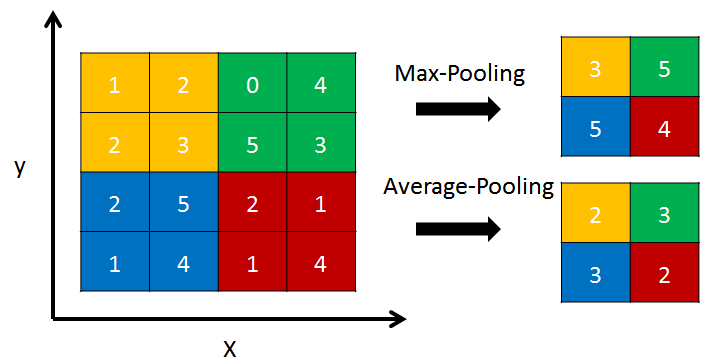
\includegraphics[scale=.8]{cnn/fig/pool.png}
	\caption{$2\times2$ pooling layer with stride 2 and padding 0.}\label{fig:cnn:pool}
\end{figure}

\subsection{Fully Connected Layer}
Fully Connected (FC) Layer have full connections to all activations in the previous layer, as seen in regular Neural Networks. Recent work show that FC layers with Rectified Linear Units and Dropout can greatly improve the learning speed as well as avoid overfitting for deep CNNs \cite{hinton2012improving} \cite{nair2010rectified}.
\subsubsection{Rectified Linear Units (ReLUs) for Activation}
Rectified Linear Units can be considered as replacing each binary unit with sigmoid activation by an infinite number of copies that all have the same weights but have progressively more negative biases. This replacing procedure can be mathematically presented as:
\begin{equation}
\sum\limits_i^N {\sigma (x - i + 0.5)}  \approx \log (1 + {e^x})
\end{equation}
where $\sigma(x)$ is the sigmoid function. In practice, Rectified Linear Units use the function 
\begin{equation}
f(x) = \max(x,0)  \approx \log (1 + {e^x})
\end{equation}\label{eq:cnn:relu}
as the activation function for approximation \cite{jarrett2009best}. With $max$ function, the derivatives of the active ($x>0$) and inactive neurons are 1 and 0 respectively.  As a result, ReLUs can speed up the learning procedure greatly and improve the performance.
\subsubsection{DropOut}
In FC layer, nodes are connected to each other and this leads to a large number of parameters. Generally, larger number of parameters means more power for Neural Networks and more easily prone to overfitting. Dropout is a technique for addressing this problem.
The key idea is to randomly drop units (along with their connections) from the neural network during training \cite{srivastava2014dropout}. Technically, dropout can be interpreted as adding extra noise into the training procedure. Without actually adding noise, FC layer with dropout is tolerant of higher level of noise (20 \%-50\%). Randomly dropping out the nodes, for any node in FC layer, it can't rely on the other nodes to adjust its result. By eliminating the co-adaptation of hidden units, dropout becomes a technique that can be applied to any general domain and improve the performance of neural nets.   
\begin{figure}
	\centering
	\begin{tabular}{cc}
		\subfloat[ Standard Neural Net ]{    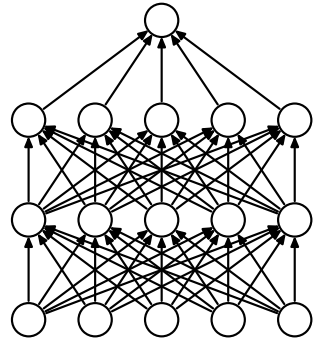
\includegraphics[width=0.3\textwidth]{cnn/fig/net.png}}&
		\subfloat[After Dropout]{    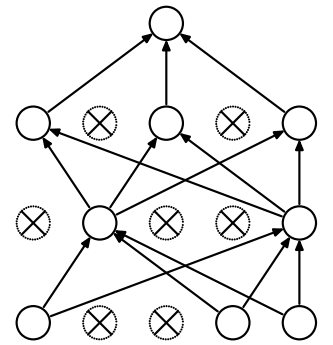
\includegraphics[width=0.3\textwidth]{cnn/fig/dropnet.png}} \\
	\end{tabular}
	\caption{Dropout Layers. Adopted from Standford CS231n Convolutional Neural Networks for Visual Recognition}
\end{figure}